%%%%%%%%%%%%%%%%%%%%%%%%%%%%%%%%%%%%%%%%%
% Diaz Essay
% LaTeX Template
% Version 2.0 (13/1/19)
%
% This template originates from:
% http://www.LaTeXTemplates.com
%
% Authors:
% Vel (vel@LaTeXTemplates.com)
% Nicolas Diaz (nsdiaz@uc.cl)
%
% License:
% CC BY-NC-SA 3.0 (http://creativecommons.org/licenses/by-nc-sa/3.0/)
%
%%%%%%%%%%%%%%%%%%%%%%%%%%%%%%%%%%%%%%%%%

%----------------------------------------------------------------------------------------
%	PACKAGES AND OTHER DOCUMENT CONFIGURATIONS
%----------------------------------------------------------------------------------------
\documentclass[11pt]{diazessay} % Font size (can be 10pt, 11pt or 12pt)
\usepackage{graphicx}
\usepackage{array}
\usepackage{tabularx}
\usepackage{float}
\usepackage{csquotes}
\usepackage{csquotes}
\usepackage{listings}
\usepackage{xcolor}
\usepackage{amsmath}
\lstset { %
    language=C++,
    backgroundcolor=\color{black!5}, % set backgroundcolor%
    basicstyle=\footnotesize,% basic font setting
    breaklines=true,
}
%----------------------------------------------------------------------------------------
%	TITLE SECTION
%----------------------------------------------------------------------------------------

\title{\textbf{Trabajo Práctico} \\ {\Large\itshape Analisis de Circuitos}} % Title and subtitle

\author{\textbf{Cotarelo Rodrigo} \\ \textit{Facultad de Ingeniería, Universidad de Buenos Aires}} % Author and institution

\date{\today} % Date, use \date{} for no date



%----------------------------------------------------------------------------------------

\begin{document}

\vbox{
    \centering
    \maketitle %this typesets the contents of \title, \author and \date
    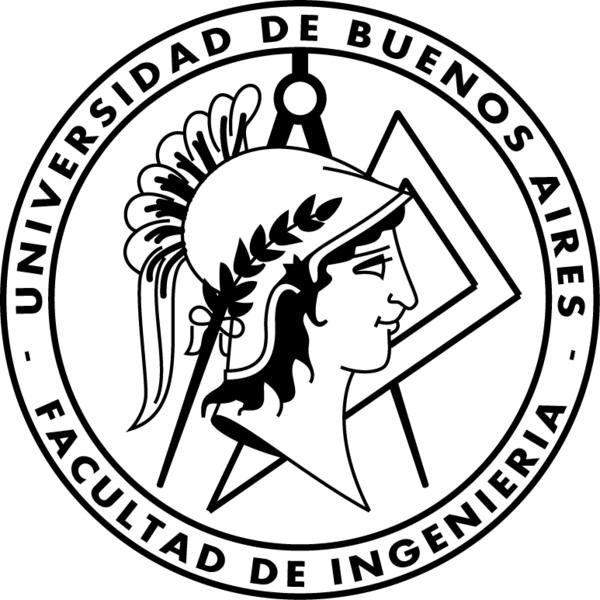
\includegraphics[width=0.5\textwidth]{Figures/fiuba.png}
}


%----------------------------------------------------------------------------------------
%	ESSAY BODY
%----------------------------------------------------------------------------------------
\newpage
\section*{Definir tipo de filtro}

\begin{equation}
H(s) = \frac{6,317 \cdot 10^8 \cdot s^2}{s^4 + 3,554 \cdot 10^4 \cdot s^3 + 1,895 \cdot 10^9 \cdot s^2 + 2,245 \cdot 10^{13} \cdot s + 3,99 \cdot 10^{17}} 
\end{equation}

En un primer analisis podemos indentificar que se trata de un filtro pasa-banda ya que tendiendo a infinito o menos infinito podemos 
ver que la transferencia es cero. Ademas como tenemos un cero en cero sabemos que hay una subida de ganancia que luego tiene que ser atenuada y es por esto
que lo podemos diferenciar de un pasa-bajos por ejemplo.\\
\\
Esta compuesto por 4 polos los cuales son dos pares complejos conjugados:
\begin{itemize}
	\item -12002.32+34212.9j\\
	\item -12002.32-34212.9j\\
	\item -5767.68+16439.38j\\
	\item -5767.68-16439.38j
\end{itemize}

Como los polos complejos conjugadores se consideran como un polo real doble y sabiendo como se conforma el diagrama asintotico sabemos que existen
dos caidas en la transferencia (una por cada polo doble) con pendiente -40db y una subida de 40db gracias al cero doble. Esto se corresponde con el
grafico de pasabanda que esperamos obtener.

La transferencia puede expresarse como la multiplicacion de dos transferencia de orden dos como se muestra a continuacion:
\begin{equation}
H(s) = H_{0} \cdot \frac{ 2 \cdot \alpha_{1} \cdot s }{ s^2 + 2 \cdot \alpha_{1} \cdot s + w_{1}^2} \cdot \frac{ 2 \cdot \alpha_{2} \cdot s }{ s^2 + 2 \cdot \alpha_{2} \cdot s + w_{2}^2}
\end{equation}
\begin{itemize}
\item Expresion pasa-bandas 2 orden:
\begin{equation}
H = \frac{ 2 \cdot \alpha \cdot s }{ s^2 + 2 \cdot \alpha \cdot s + w^2}
\end{equation}
\begin{equation}
Q = \frac{w}{2 \cdot \alpha}
\end{equation}
\begin{equation}
f = \frac{w}{2 \cdot \pi}
\end{equation}\\
\item El primer pasa-bandas de orden 2:
\begin{equation}
H_{1} = \frac{24004.64 \cdot s}{s^2 + 24004.6 \cdot s + 1314578211.7924} 
\end{equation}
$\alpha_{1}$ = 12002.32\\
$w_{1}$ = 36257.11\\
$f_{1}$ = 5770.5\\
$Q_{1}$ = 1.51\\
\item El segundo pasa-bandas de orden 2:
\begin{equation}
H_{2} = \frac{11535.36 \cdot s}{s^2 +11535.36 \cdot s + 303519347.3668} 
\end{equation}
$\alpha_{2}$ = 5767.68\\
$w_{2}$ = 17421.81\\
$f_{2}$ = 2772.77\\
$Q_{2}$ = 1.51\\
\item Comparando las transferencias
\begin{equation}
6,317 \cdot 10^8 = H_{0} \cdot 2\alpha_{1} \cdot 2\alpha_{2}
\end{equation}
\begin{equation}
H_{0} = 2.28\\
\end{equation}
\end{itemize}
El polo con la parte real mas chica (en este caso $\alpha_{2}$ = 5767) es el que estabiliza el sistema, por lo tanto $\tau$ = $\frac{1}{\alpha_{2}}$ = 1.73 $\cdot$ 10$^{-4}$ y nuestro ciruitos se estabilizaria a los 0.86ms (5 $\cdot$ $\tau$)\\


\newpage
\section*{Simulacion}
\begin{itemize}
\item Diagrama de Bode de modulo y fase \\
Podemos confirmar lo explicado anteriormente. El gráfico muestra claramente la subida de 40 db por década que después se compensa con el primer polo doble generando una meseta y en el segundo polo doble se produce la caída de -40 db por década.\\
\begin{figure}[h]
	\centering
	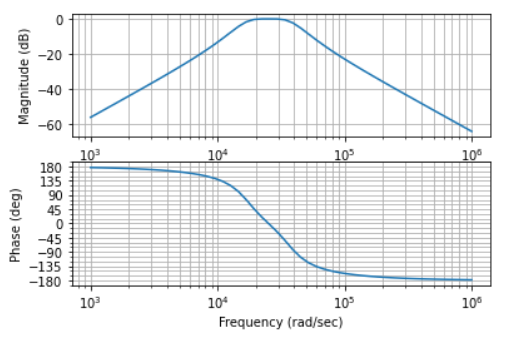
\includegraphics[width=\textwidth]{Bode.png}
\caption{Diagrama de Bode de modulo y fase}
\end{figure}\\
\newpage
\item Respuesta al escalon\\
En la respuesta al escalon primero tenemos un flanco ascendente y despues una continua. En el flanco ascendente al tener un pasabanda que filtra las frecuencia altas esperamos que no suba de golpe y una vez que termine el transitorio tiene que tender a cero ya que al filtrar las frecuencias bajas no estamos dejando pasar la componente continua.
\begin{figure}[h]
	\centering
	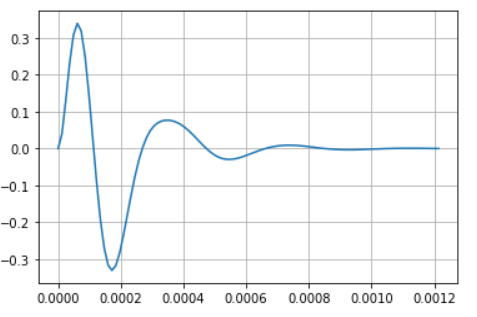
\includegraphics[width=\textwidth]{Respuesta_al_escalon.png}
\caption{Respuesta al escalon.}
\end{figure}
\newpage
\item Respuesta al impulso
\begin{figure}[h]
	\centering
	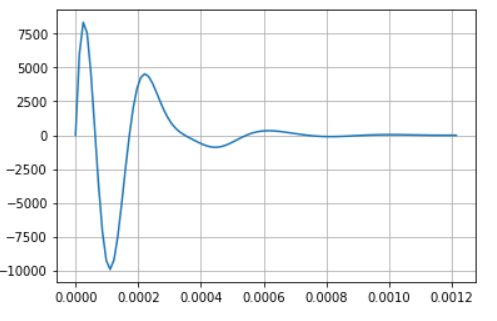
\includegraphics[width=\textwidth]{Respuesta_al_impulso.png}
\caption{Respuesta al impulso.}
\end{figure}
\item Respuesta a la senoidal \\
\\
Al tener un filtro pasabanda vamos a utilizar una frecuencia f0 = 4200Hz que esta dentro de nuestro ancho de banda y esperamos que el filtro atenue las senionadales con frecuencia de 1 decada mayor y menor.
\begin{figure}[h]
	\centering
	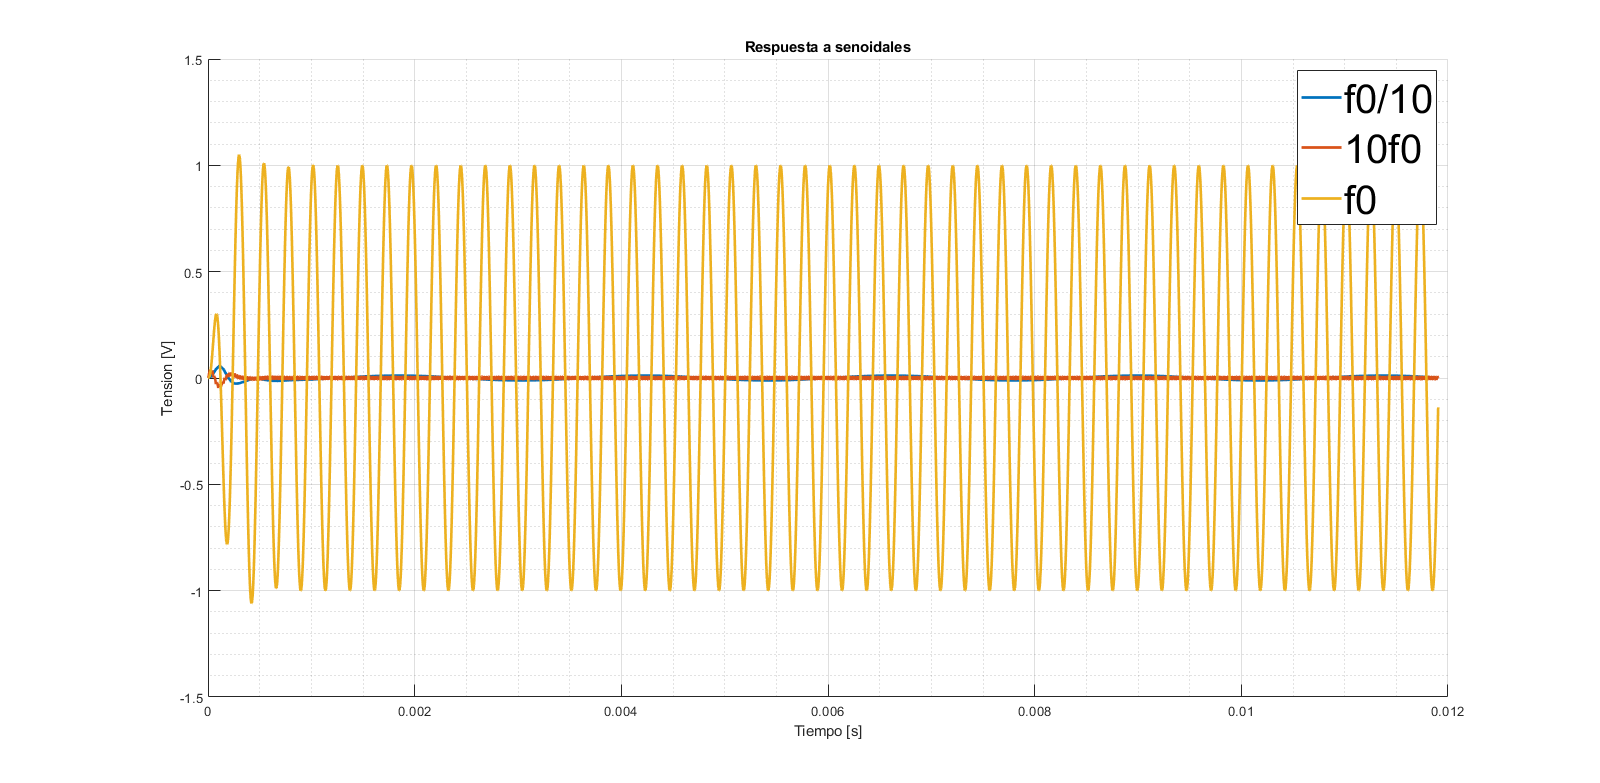
\includegraphics[width=\textwidth]{Respuesta_senoidal.png}
\caption{Respuesta a señal senoidal.}
\end{figure}
\newpage
\item Respuesta a la cuadrada
\begin{itemize}
\item f0 = 4200 Hz \\
Para este caso tenemos una cuadrada con periodo de $\frac{1}{f}$ = 2.38 $\cdot$ 10$^{-4}$s, menor a 5 $\cdot$ $\tau$, por lo que vamos a ver solo una parte del transitorio. En cada flanco ascendete el filtro va a responder subiendo suavemente ya que estamos filtrando las frecuencias altas que forman al flanco, despues viene la parte plana de la cuadrada (frecuencias bajas) que tambien es filtrada por lo que el grafico va a caer suavemente tambien.Finalmente el flanco decendente se encarga de repetir la misma parte inicial del transitorio pero invirtiendo el comportamiento. Como filtra las frecuencias bajas, se va a filtrar la componente continua de esta cuadrada que es 0.5 (valor medio) por lo que  la salida deberia tener una continua cero.
	\begin{figure}[h]
		\centering
			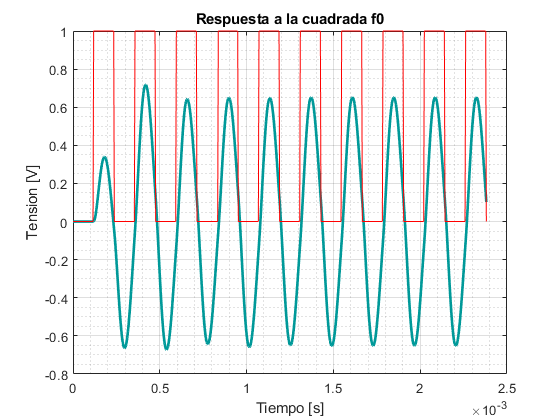
\includegraphics[width=\textwidth]{cuadrada_f0.png}
	\caption{Respuesta cuadrada.}
	\end{figure}
\newpage
\item f0/10 \\
Para la segunda cuadrada con periodo de $\frac{1}{420}$ = 2.38ms que es claramente mayor a los 0.86 que necesita nuestro filtro para estabilizarse. Por lo tanto como en cada periodo el circuito llega a estabilizarse, vamos a poder ver en cada flanco ascendete la forma de la respuesta al escalon completa mientras que en los flancos descendientes la misma forma invertida.
	\begin{figure}[h]
		\centering
			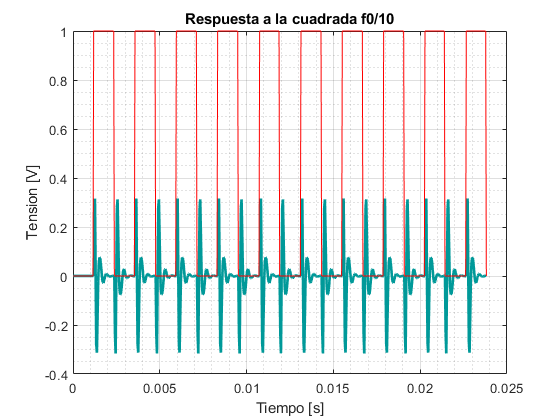
\includegraphics[width=\textwidth]{cuadrada_f0_div_10.png}
	\caption{Respuesta cuadrada.}
	\end{figure}
\newpage
\item 10 $\cdot$ f0 \\
Esta cuadrada es la de menor periodo ($\frac{1}{42000}$ = 23.8us) por lo que veremos una menor parte del transitorio todavia.
	\begin{figure}[h]
		\centering
			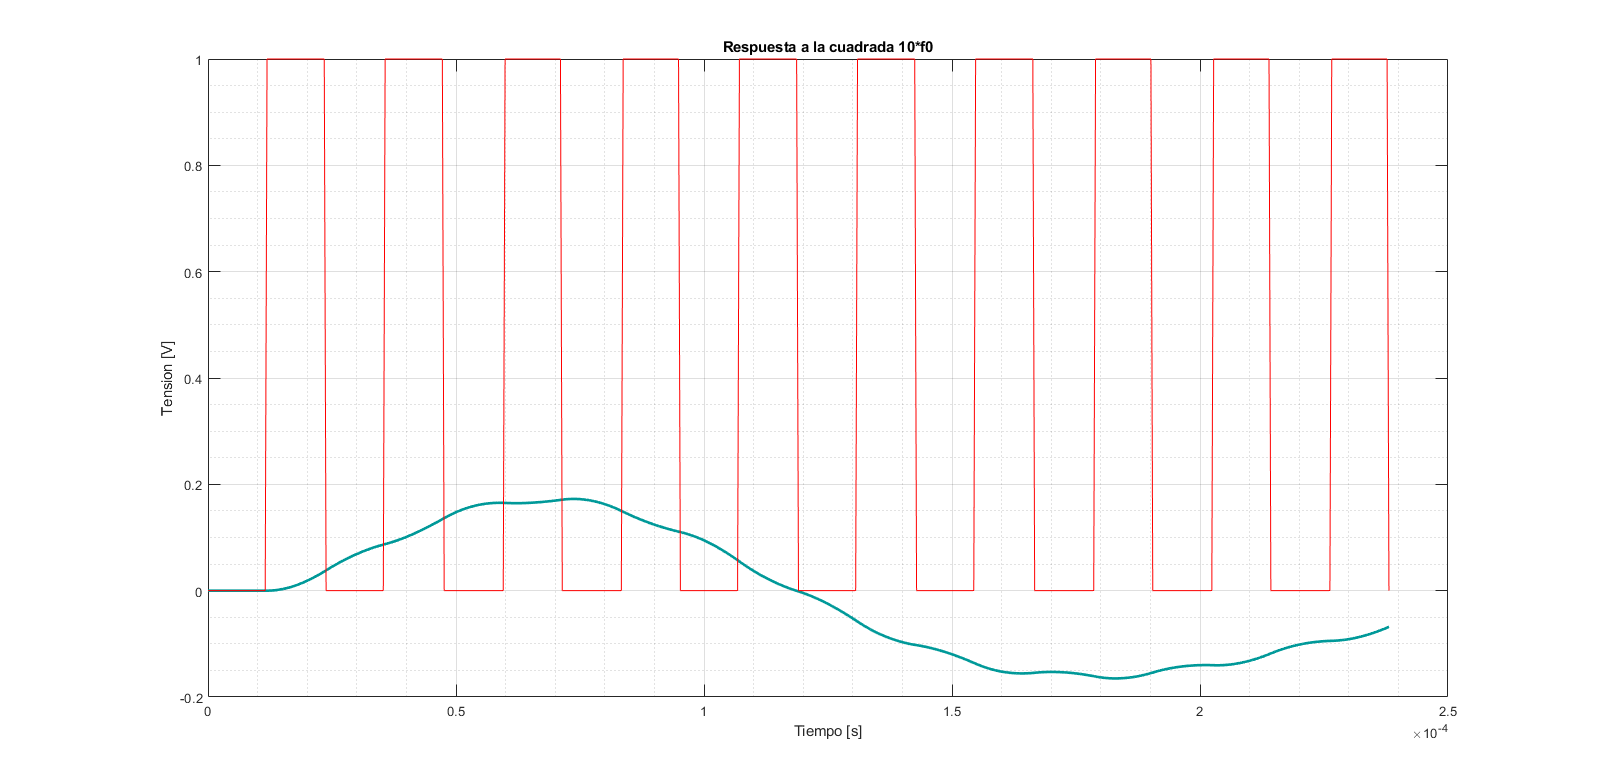
\includegraphics[width=\textwidth]{cuadrada_f0_por_10.png}
	\caption{Respuesta cuadrada.}
	\end{figure}
	\begin{figure}[h]
		\centering
			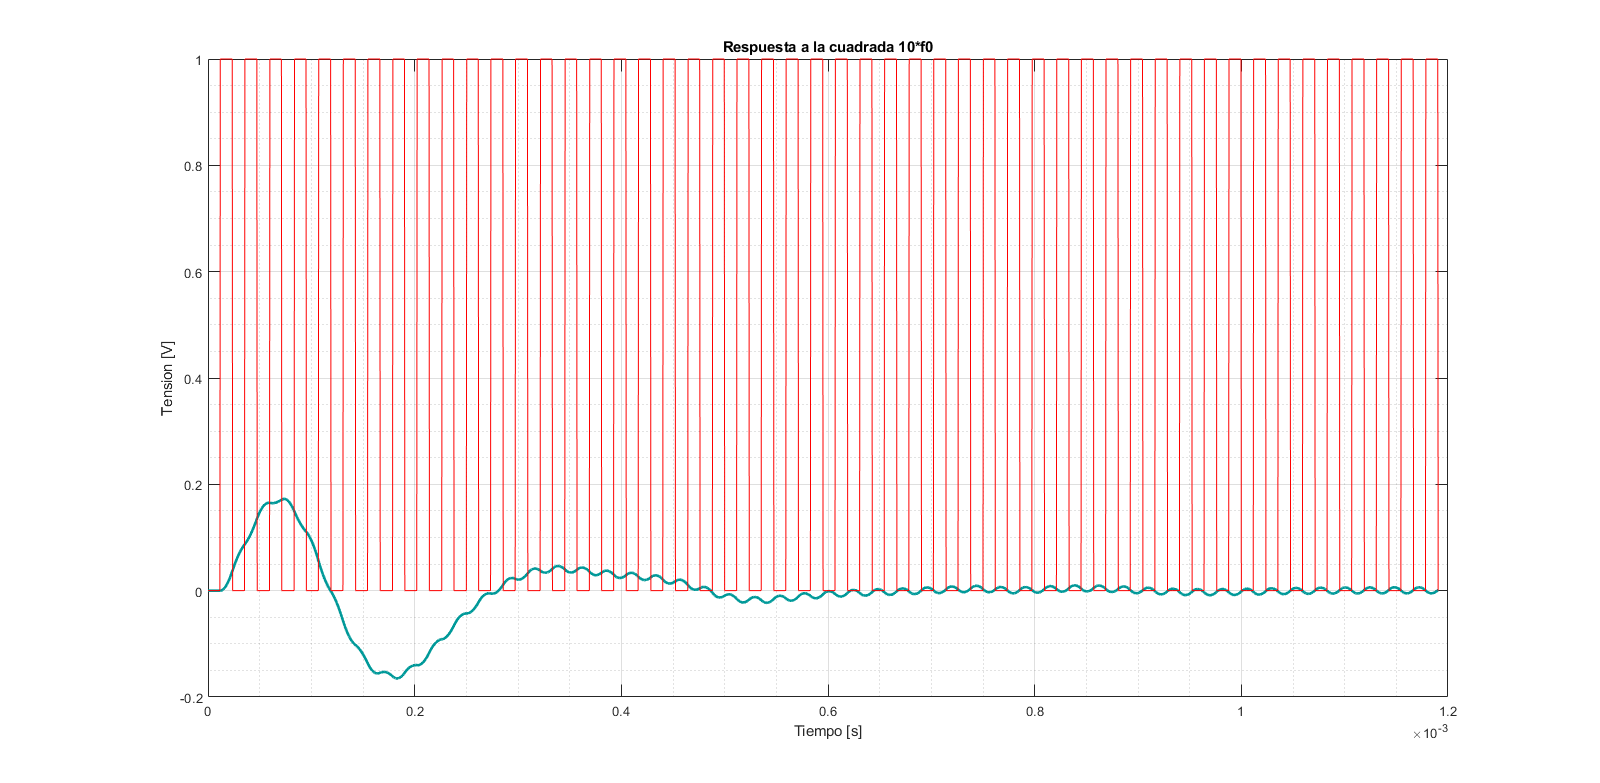
\includegraphics[width=\textwidth]{cuadrada_f0_por_10_v2.png}
	\caption{Respuesta cuadrada con mas periodos.}
	\end{figure}

\end{itemize}
\end{itemize}

\newpage
\section*{Eleccion de circuito}
Para implementar este filtro se usaron dos pasabandas "Infinite Gain Multiple Feedback" conectados en cascada por las siguientes razones: \\
\begin{itemize}
\item Permite trabajar con cualquier factor de calidad Q.\\
\item Al implementar dos IGMF lograba alcanzar la ganancia deseada conectando solamente dos de ellos en cascada. En caso de utilizar un pasabajos y pasaltos corria el riesgo de tener que agregar un tercer ciruito en cascada (agregar mas componentes) para lograr la ganancia deseada.\\
\item El diseño me permitia usar pocos componentes.\\
\item Ya lo habiamos trabajado en clase.
\end{itemize}
\begin{figure}[h]
\centering
	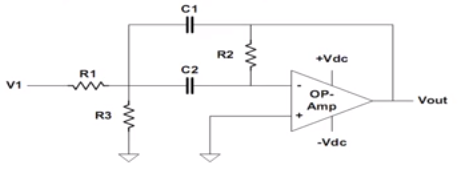
\includegraphics[width=\textwidth]{filtro.png}
\caption{Infinite Gain Multiple Feedback}
\end{figure}

Las ecuaciones de este circuito son las siguientes:

\begin{align*}
H(s) &= -H_{0} \frac{ \frac{w_{0}}{Q} \cdot s }{ s^{2} + \frac{w_{0}}{Q} \cdot s + w_{0}^{2} } \\[10pt]
C_{1} &= C_{2} = C \\[10pt]
H_{0} &= \frac{R_{2}}{2 \cdot R_{1}} \\[10pt]
\frac{w_{0}}{Q} &= \frac{2}{C \cdot R_{2}} \\[10pt]
w_{0}^{2} &= \frac{ 1 + \frac{R_{1}}{R_{3}} }{ C^{2} \cdot R_{1} \cdot R_{2} }
\end{align*}

\newpage
\begin{align*}
R_{2} &= \frac{2 \cdot Q}{ C \cdot w_{0} } \\[10pt]
R_{1} &= \frac{ R_{2} }{ 2 \cdot H_{0} } \\[10pt]
R_{3} &= \frac{ R_{1} }{ \frac{2 \cdot Q^{2} }{ H_{0} } - 1 }
\end{align*}

Con estos datos se diseño el filtro como dos IGMB en cascada. Para ambos se busco un $H_{0}$ de 1.51 para lograr el de 2.28 y como en cada uno sabiamos $H_{0}$, Q y f solo quedaba buscar definir un valor de C para luego reemplazar y buscar los valores de resistencias necesarios.
\newpage
\section*{Valores normalizados}
En base a las ecuaciones del circuito presentadas arriba se calcularon los valores necesarios de los componentes junto a sus valores
normalizados respectivamente.\\
\break
\begin{tabular}{ |p{2cm}||p{2cm}|p{6cm}|  }
 \hline
 \multicolumn{3}{|c|}{Filtro pasabajos 1} \\
 \hline
 Componente&Valor&Valor Normalizado\\
 \hline
 C  & 12nF & 12nF\\
 R2  & 6.94k & 6.8k\\
 R1  & 2.30k & 2.2k\\
 R3  & 1.13k & 1.2k\\
 \hline
\end{tabular}\\
\break
\break
\begin{tabular}{ |p{2cm}||p{2cm}|p{6cm}|  }
 \hline
 \multicolumn{3}{|c|}{Filtro pasabajos 2} \\
 \hline
 Componente&Valor&Valor Normalizado\\
 \hline
 C  & 10nF & 10nF\\
 R2  & 17.34k & 18k\\
 R1  & 5.74k & 5.6k\\
 R3  & 2.84k & 2.7k\\
 \hline
\end{tabular}
\break
\break
La transferencia obtenida con los valores normalizados es la siguiente: \\
\begin{equation}
H(s) = \frac{6,764 \cdot 10^8 \cdot s^2}{s^4 + 3,562 \cdot 10^4 \cdot s^3 + 1,893 \cdot 10^9 \cdot s^2 + 2.209 \cdot 10^{13} \cdot s + 4.011 \cdot 10^{17}} 
\end{equation}
\\
Mientras que el circuito queda de la siguiente manera: \\
\begin{figure}[h]
\centering
	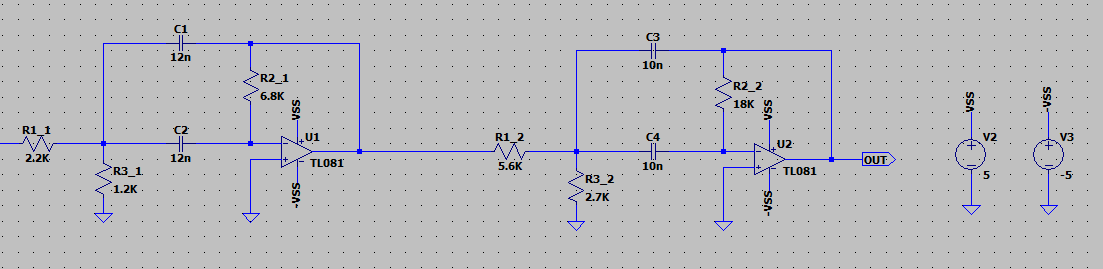
\includegraphics[width=\textwidth]{circuito_real.png}
\caption{Diagrama de bode (modulo y fase) normalizado}
\end{figure}


\newpage
\section*{Diagramas normalizados}
\begin{figure}[h]
\centering
	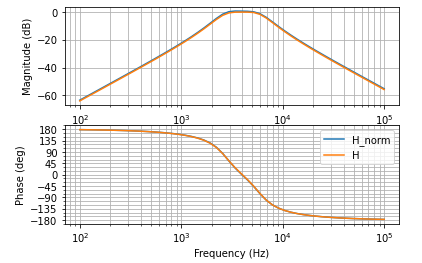
\includegraphics[width=\textwidth]{bode_norm.png}
\caption{Circuito con componentes normalizados}
\end{figure}

\begin{figure}[h]
\centering
	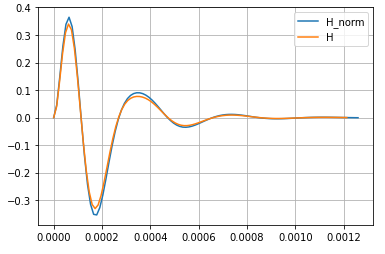
\includegraphics[width=\textwidth]{escalon_norm.png}
\caption{Respuesta al escalon normalizado}
\end{figure}

\newpage
\section*{Simulacion LTspice}
\begin{itemize}
\item Diagrama de Bode de modulo y fase
\begin{figure}[h]
\centering
	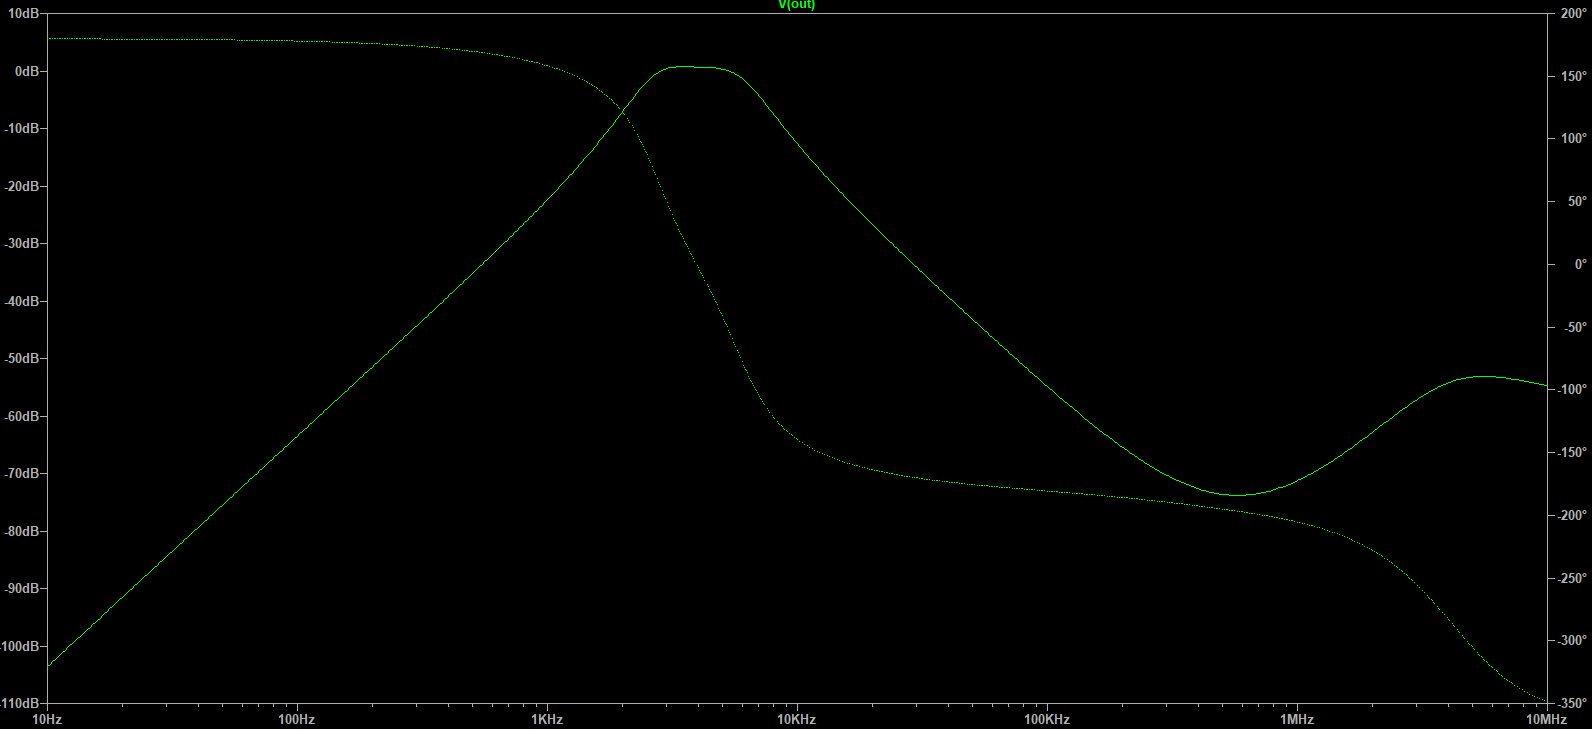
\includegraphics[width=\textwidth]{bode_TL081.png}
\caption{Diagrama de Bode ltspice}
\end{figure}

\newpage
\item Respuesta al escalon
\begin{figure}[h]
\centering
	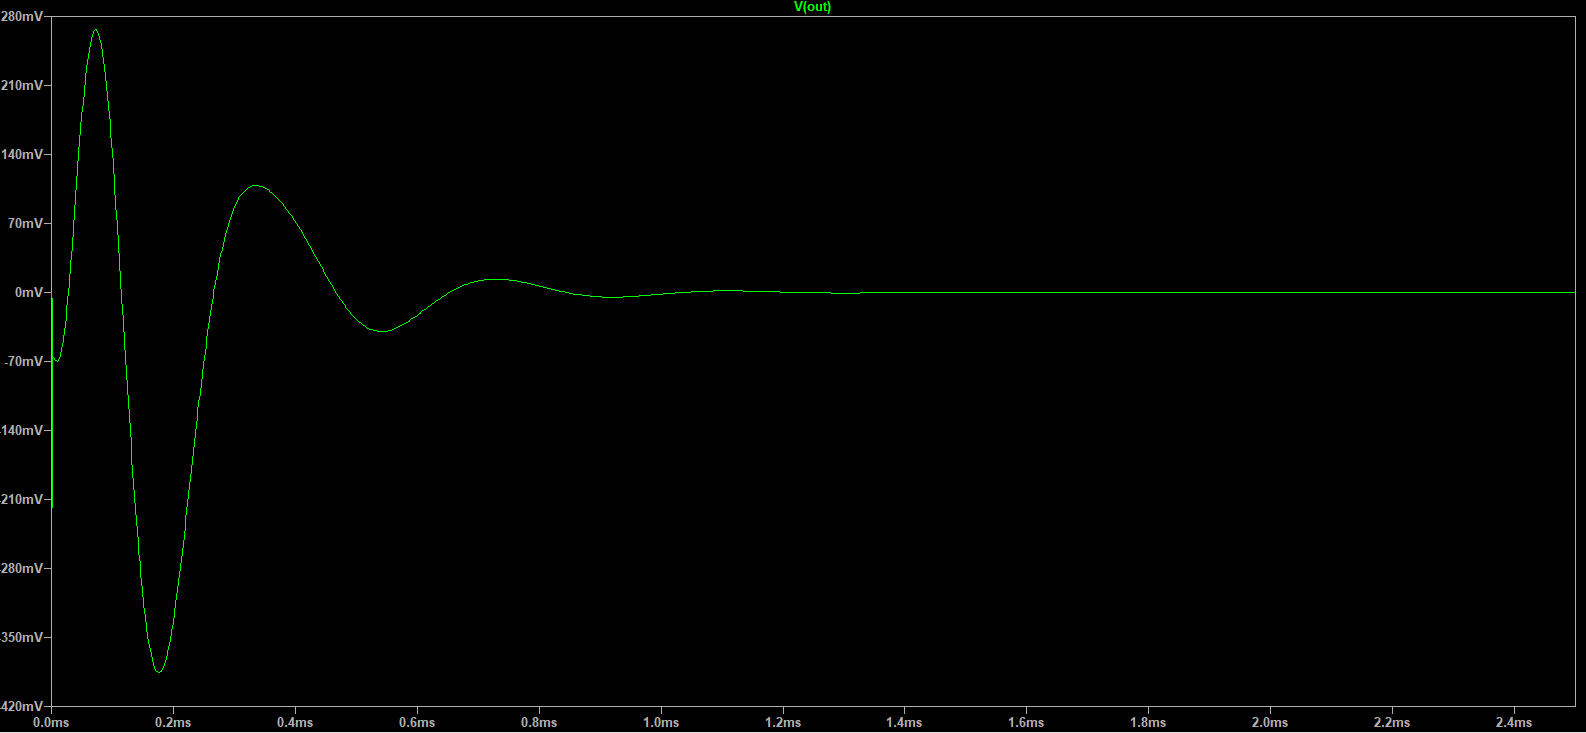
\includegraphics[width=\textwidth]{escalon_TL081.png}
\caption{Diagrama de Bode ltspice}
\end{figure}

\newpage
\begin{figure}[h]
\centering
	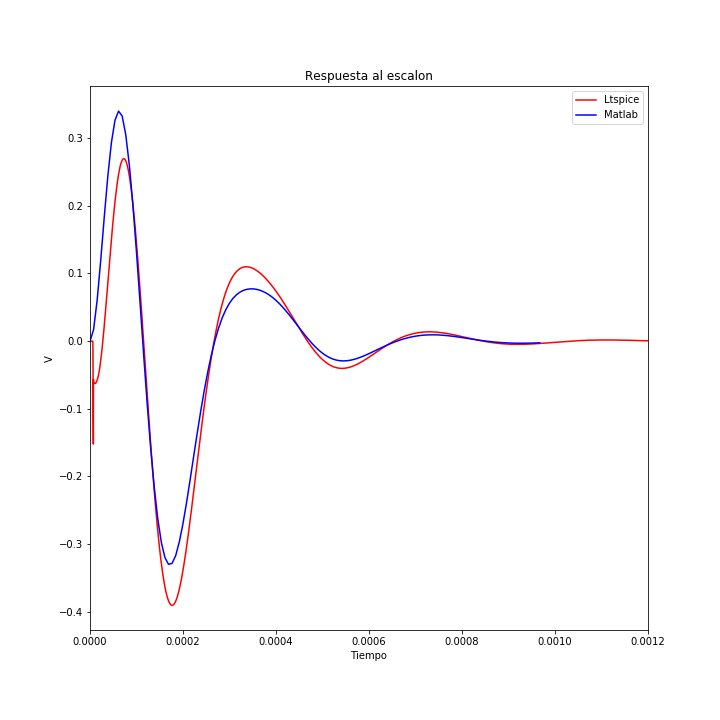
\includegraphics[width=\textwidth]{c_respuesta_escalon.png}
\caption{Simulacion LTspice normalizado vs Matlab}
\end{figure}
Este grafico es el unico que presenta corrimiento en el eje y debido al parametros de configuracion del LTspice para lograr simular la entrada de escalon que genera ruido. \\

\newpage
\item Respuesta a la senoidal
\begin{itemize}
\item f0
\begin{figure}[h]
\centering
	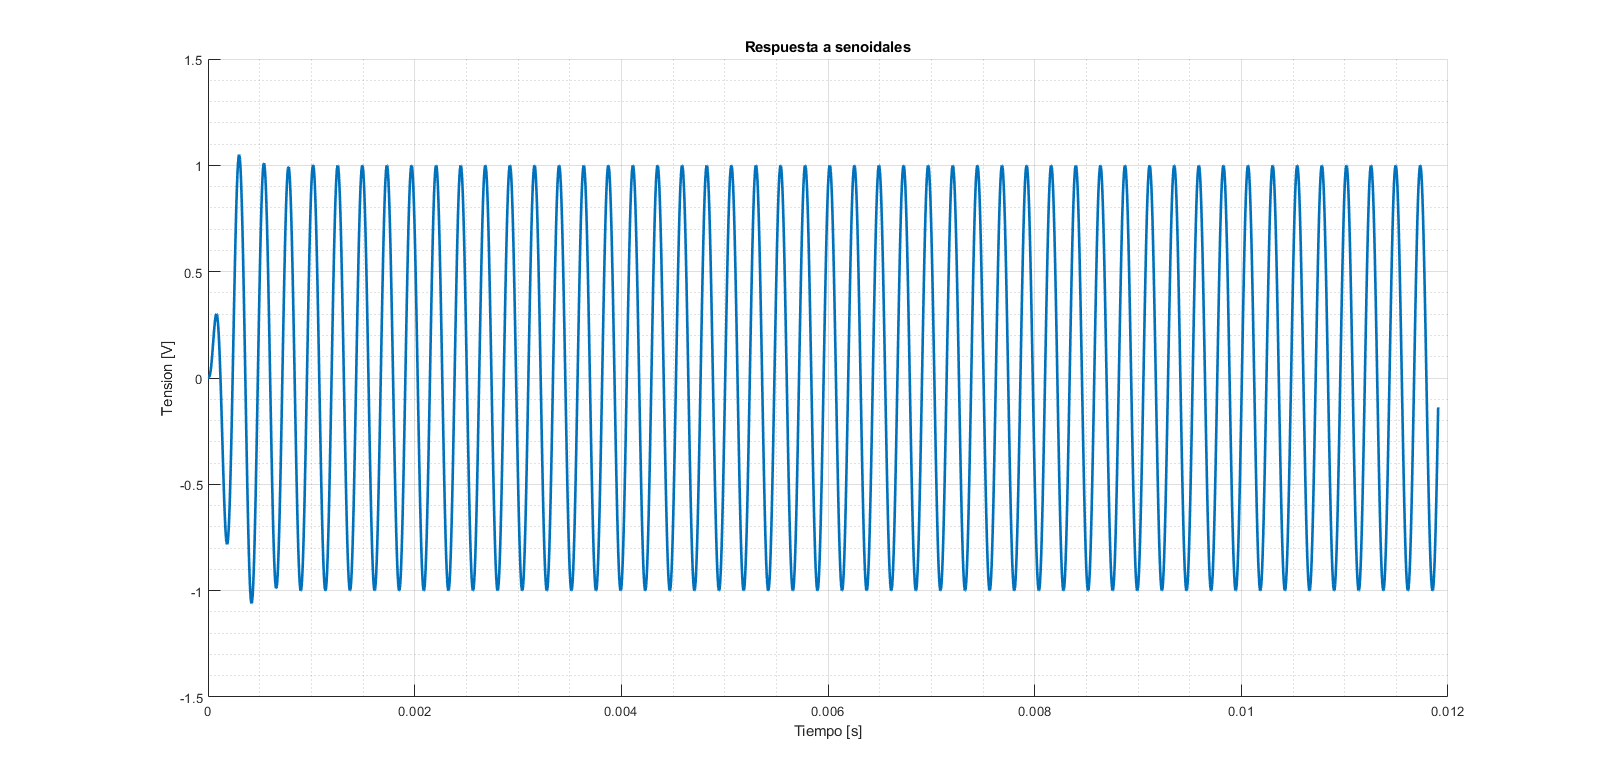
\includegraphics[width=\textwidth]{sen_fo_original.png}
\caption{Senoidal f0 original}
\end{figure}

\begin{figure}[h]
\centering
	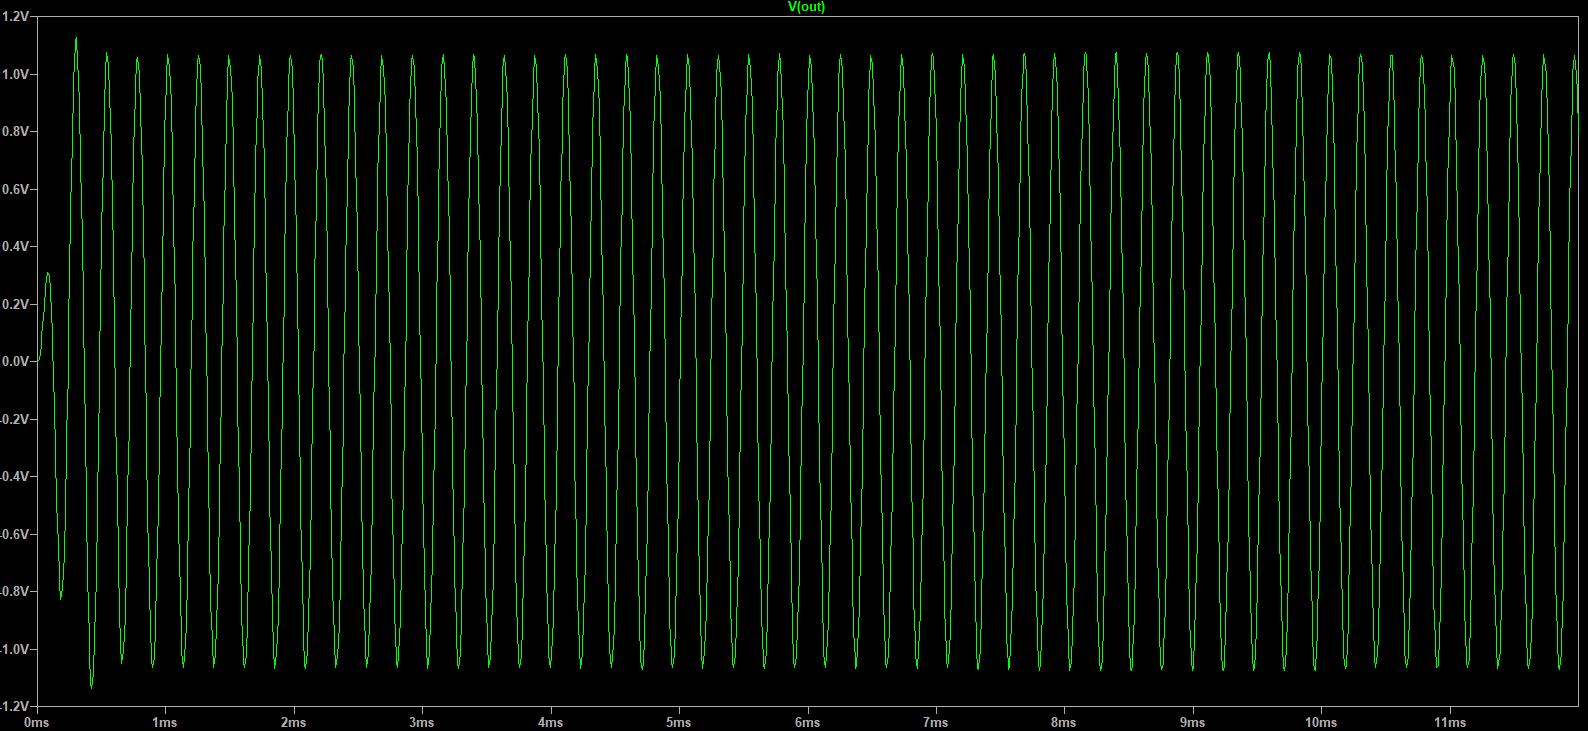
\includegraphics[width=\textwidth]{sen_fo_TL081.png}
\caption{Senoidal f0 TL081}
\end{figure}

\newpage
\begin{figure}[h]
\centering
	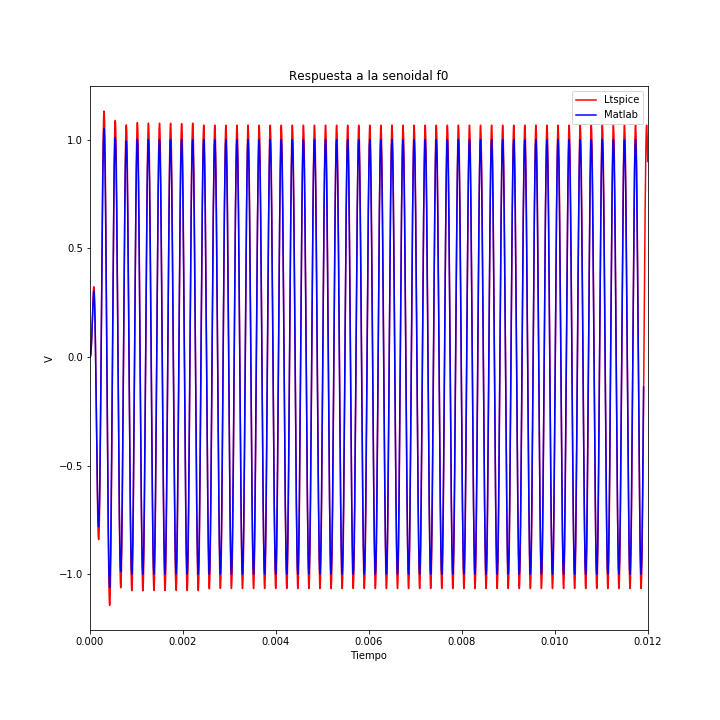
\includegraphics[width=\textwidth]{c_respuesta_senoidal_f0.png}
\caption{Simulacion LTspice normalizado vs Matlab}
\end{figure}

\newpage
\item f0/10
\begin{figure}[h]
\centering
	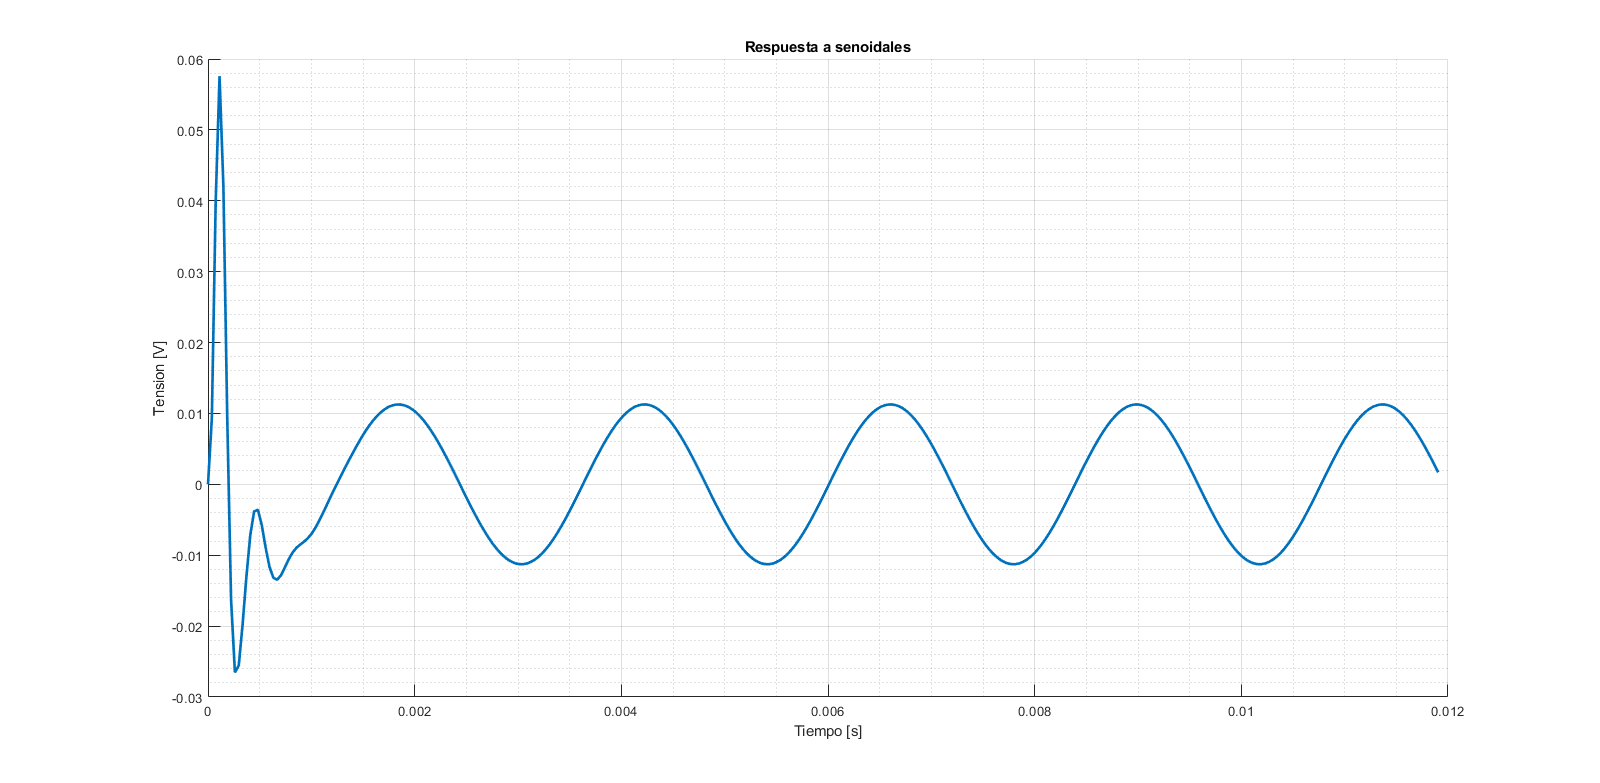
\includegraphics[width=\textwidth]{sen_fo_sobre_10_original.png}
\caption{Senoidal f0/10 original}
\end{figure}

\begin{figure}[h]
\centering
	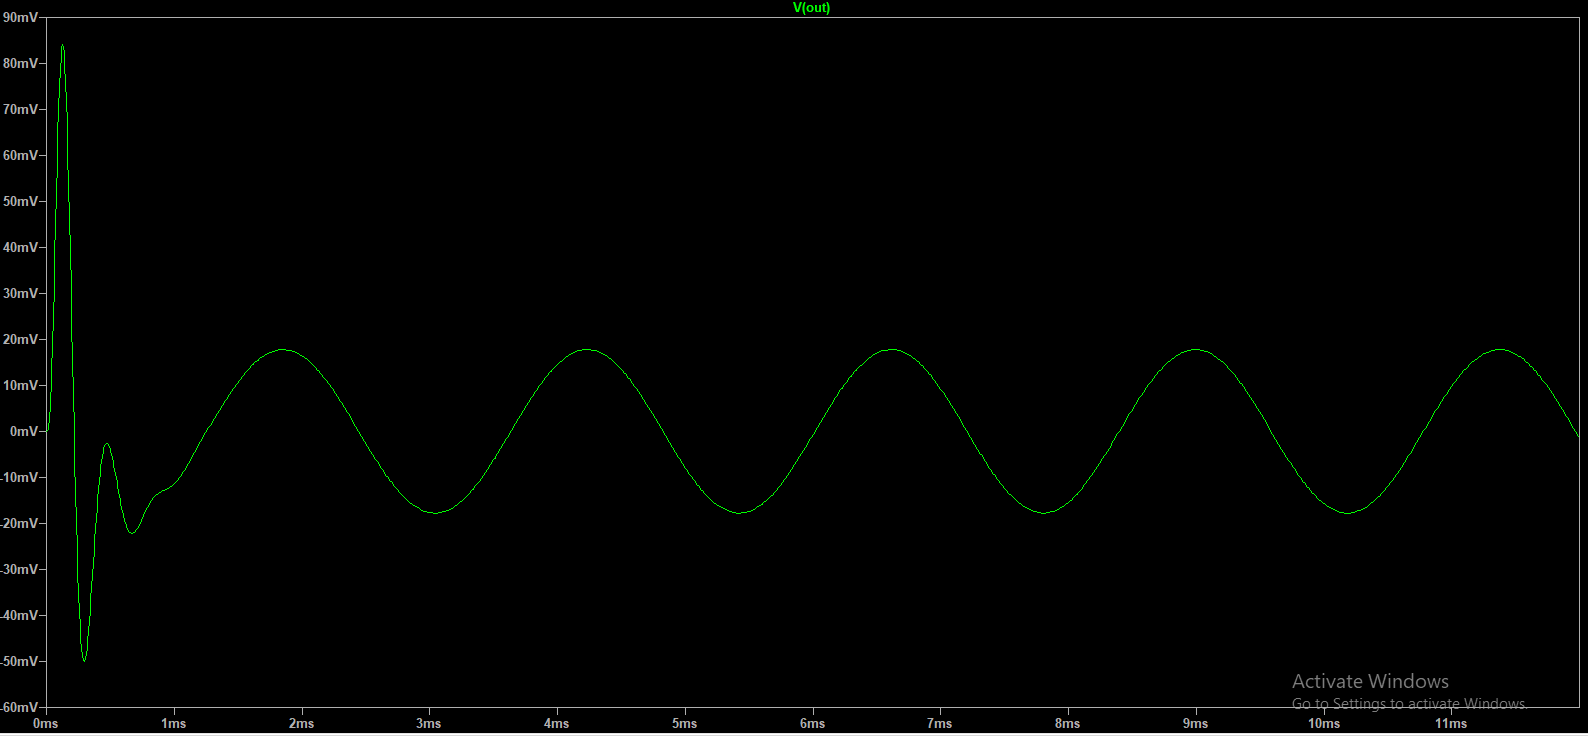
\includegraphics[width=\textwidth]{sen_fo_sobre_10_TL081.png}
\caption{Senoidal f0/10 TL081}
\end{figure}

\newpage
\begin{figure}[h]
\centering
	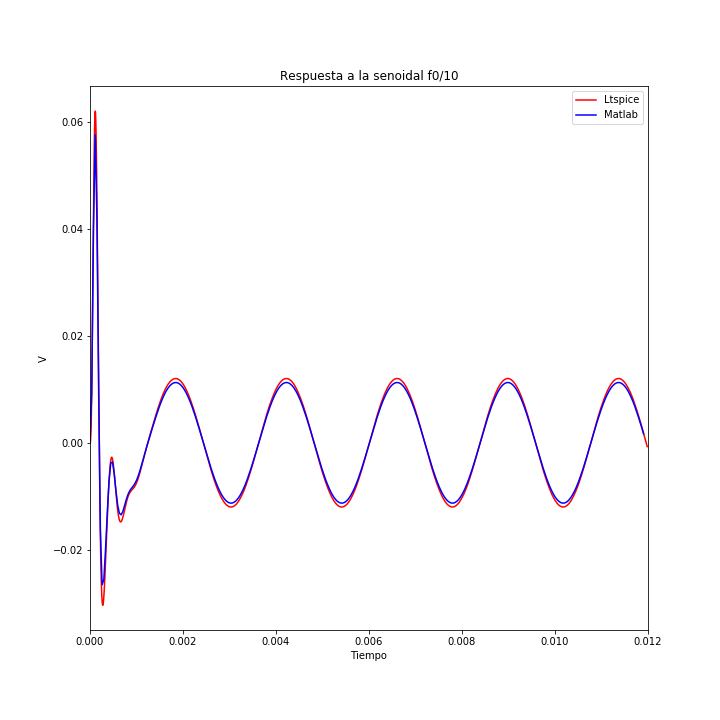
\includegraphics[width=\textwidth]{c_respuesta_senoidal_sobre_10.png}
\caption{Simulacion LTspice normalizado vs Matlab}
\end{figure}


\newpage
\item 10 $\cdot$ f0
\begin{figure}[h]
\centering
	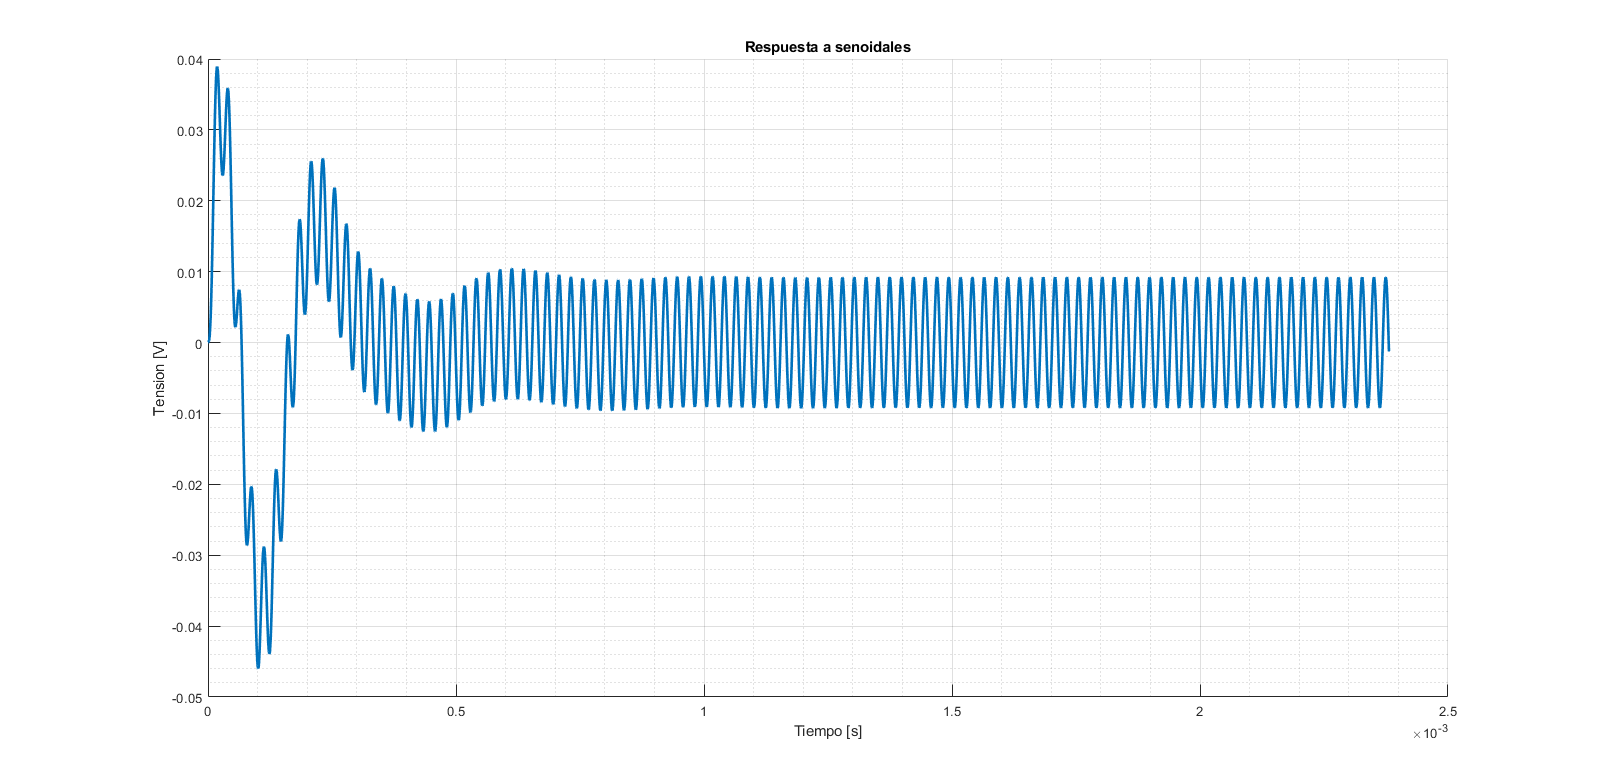
\includegraphics[width=\textwidth]{sen_fo_por_10_original.png}
\caption{Senoidal 10 $\cdot$ f0 original}
\end{figure}

\begin{figure}[h]
\centering
	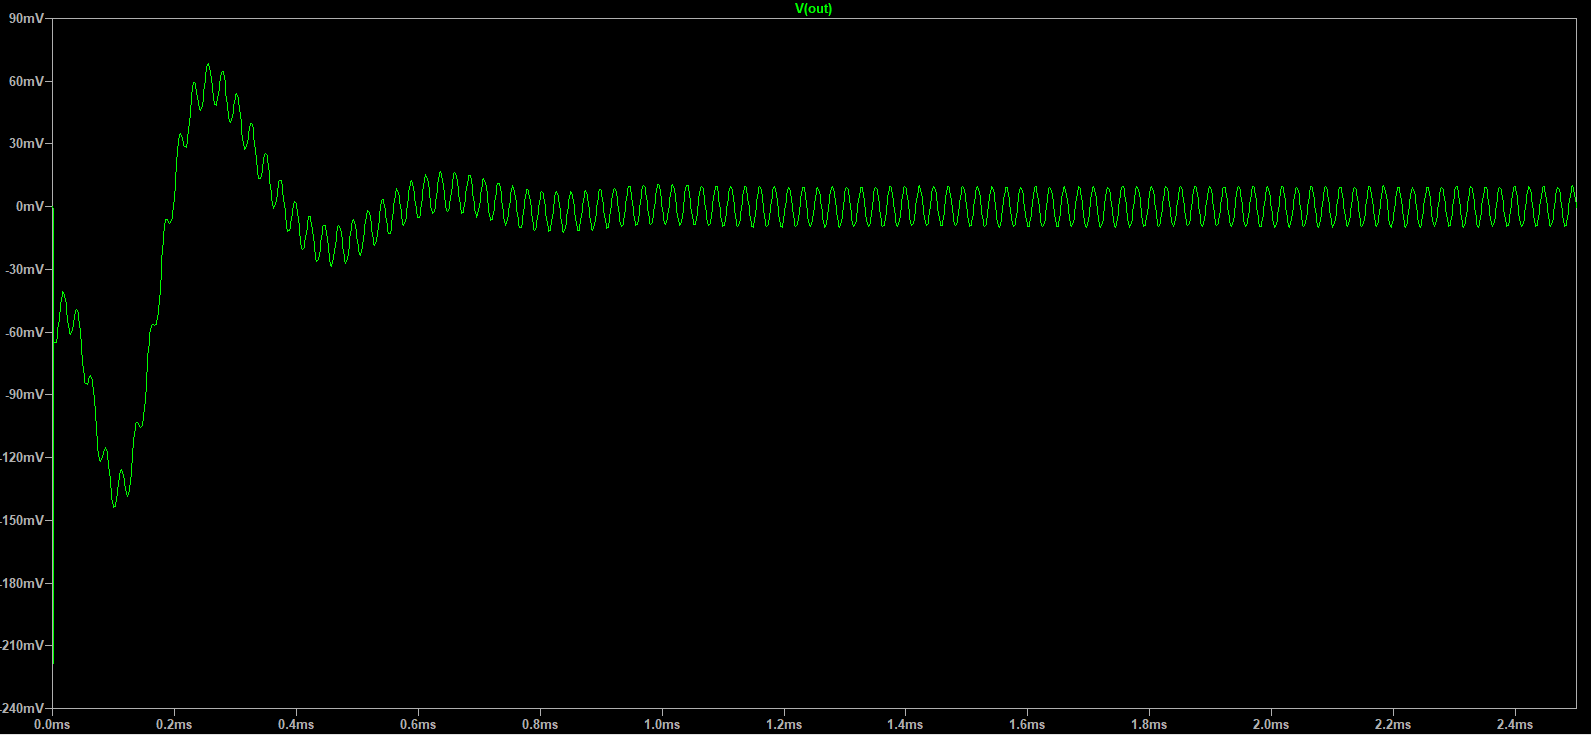
\includegraphics[width=\textwidth]{sen_fo_por_10_TL081.png}
\caption{Senoidal 10 $\cdot$ f0 TL081}
\end{figure}

\newpage
\begin{figure}[h]
\centering
	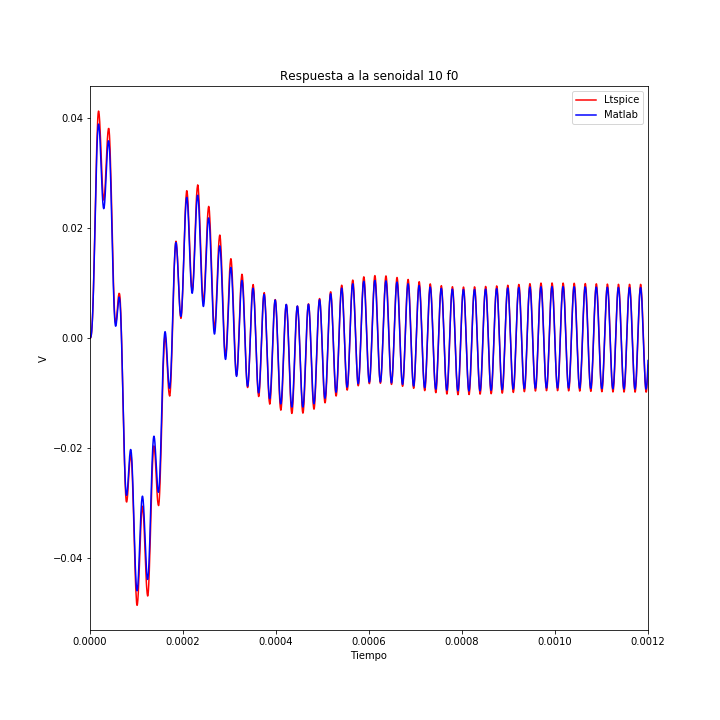
\includegraphics[width=\textwidth]{c_respuesta_senoidal_por_10.png}
\caption{Simulacion LTspice normalizado vs Matlab}
\end{figure}


\end{itemize}

\newpage
\item Respuesta a señal cuadrada
\begin{itemize}
\item f0
\begin{figure}[h]
\centering
	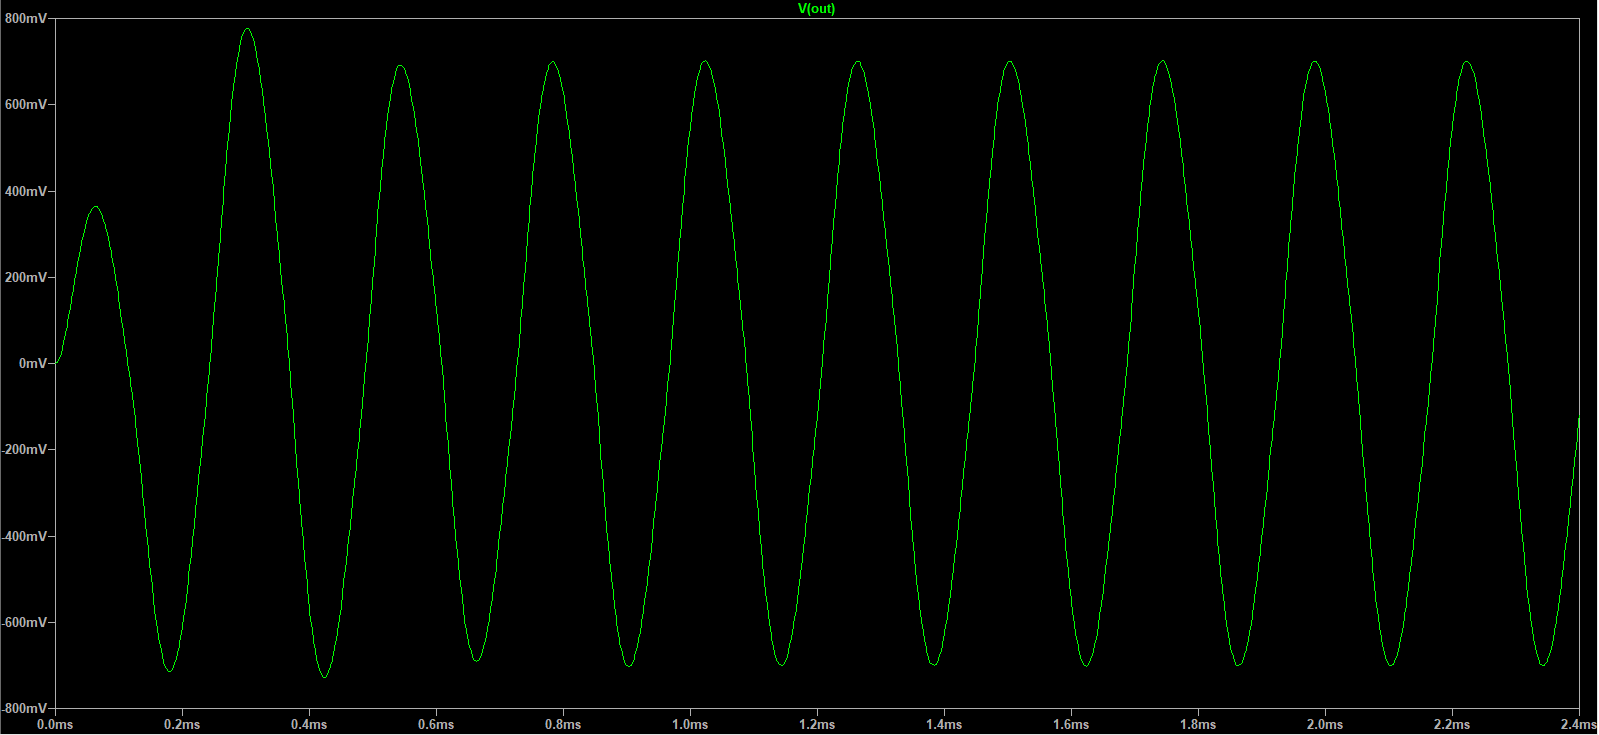
\includegraphics[width=\textwidth]{cuadrada_f0_TL081.png}
\caption{Cuadrada f0 TL081}
\end{figure}

\newpage
\begin{figure}[h]
\centering
	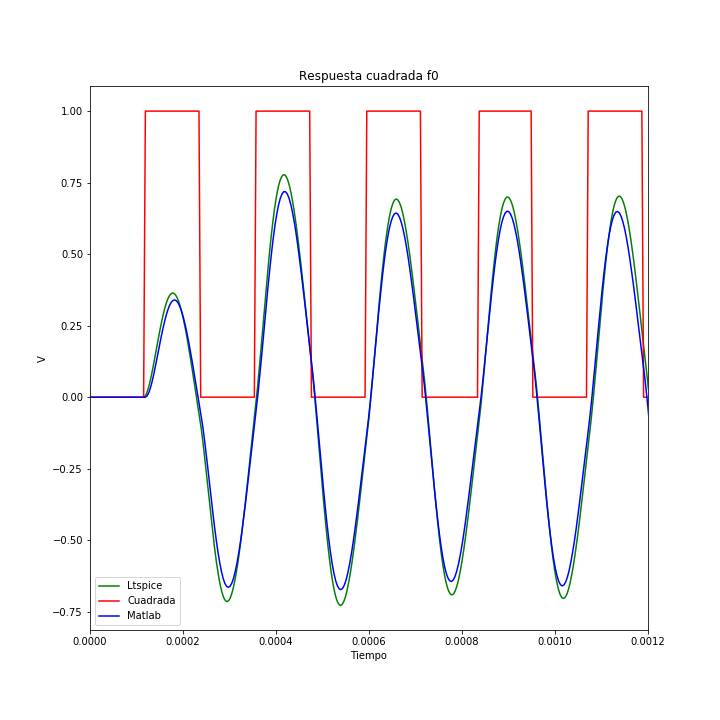
\includegraphics[width=\textwidth]{c_respuesta_cuadrada.png}
\caption{Simulacion LTspice normalizado vs Matlab}
\end{figure}


\newpage
\item f0/10
\begin{figure}[h]
\centering
	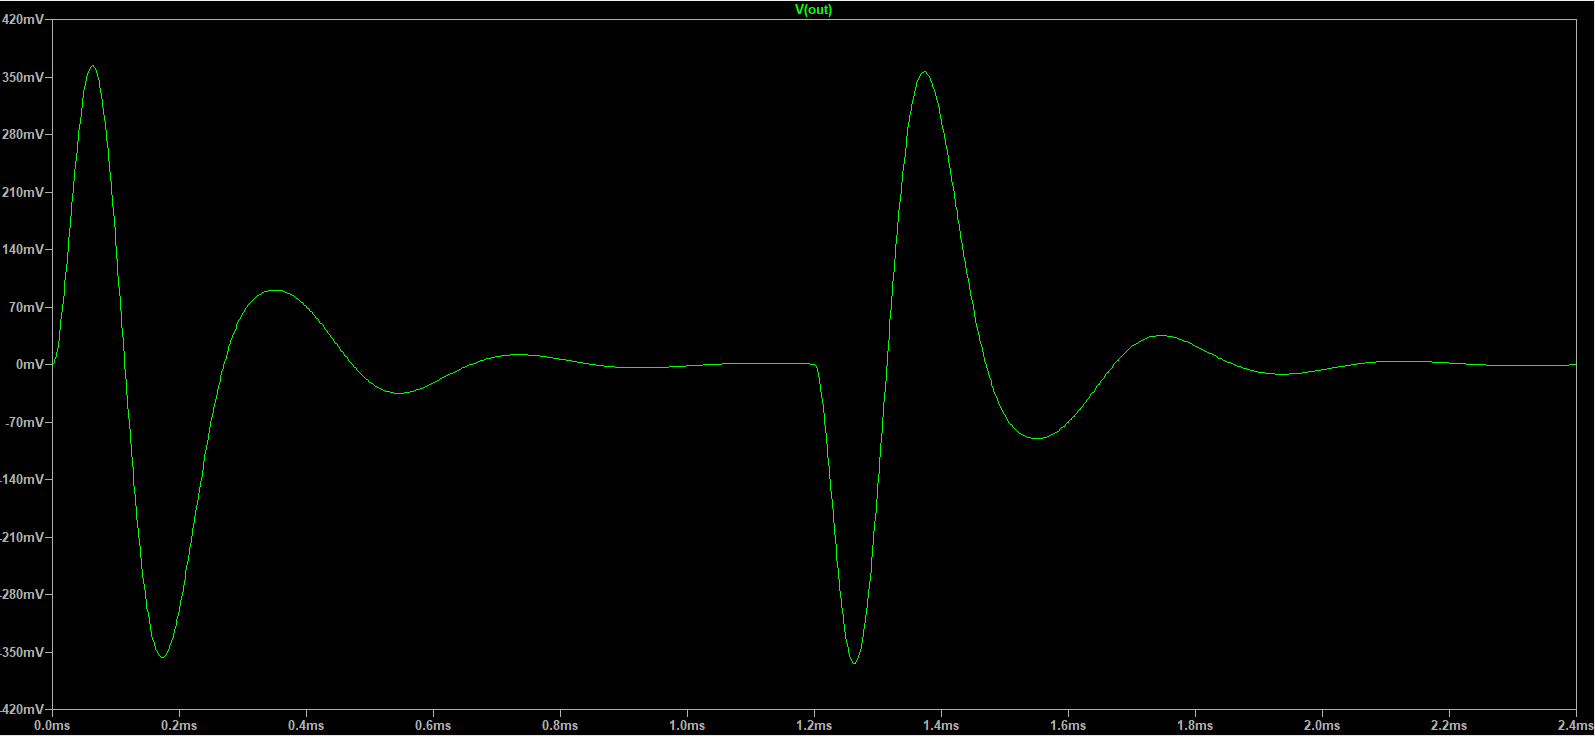
\includegraphics[width=\textwidth]{cuadrada_f0_sobre_10_TL081.png}
\caption{Cuadrada f0/10 TL081}
\end{figure}

\newpage
\begin{figure}[h]
\centering
	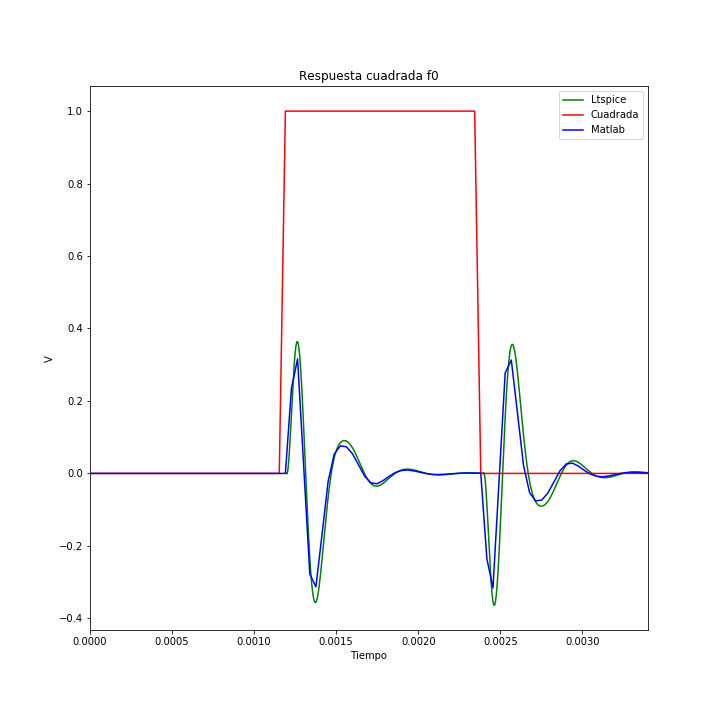
\includegraphics[width=\textwidth]{c_respuesta_cuadrada_sobre_10.png}
\caption{Simulacion LTspice normalizado vs Matlab}
\end{figure}

\newpage
\item 10 $\cdot$ f0
\begin{figure}[h]
\centering
	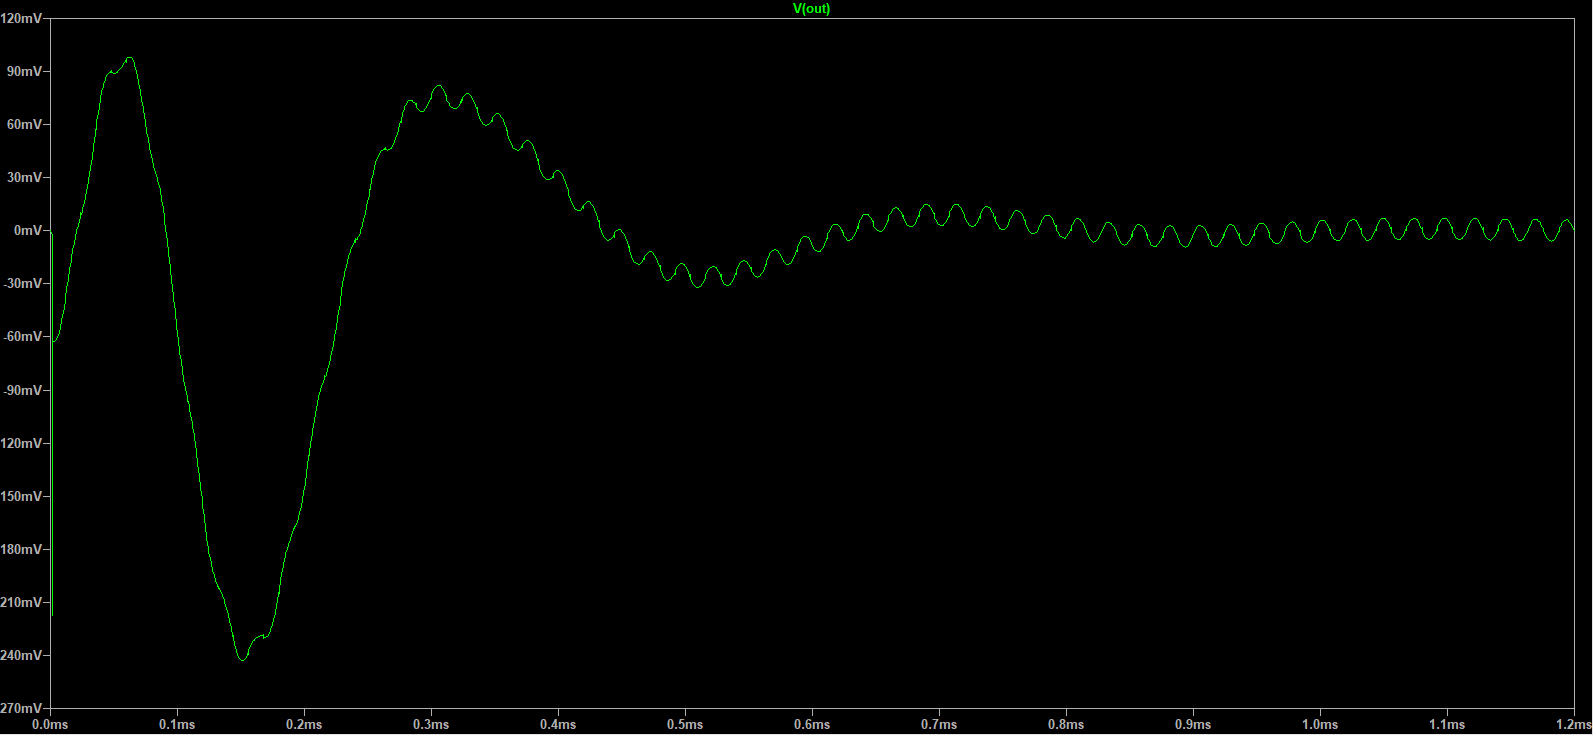
\includegraphics[width=\textwidth]{cuadrada_f0_por_10_TL081.png}
\caption{Cuadrada 10 $\cdot$ f0 TL081}
\end{figure}

\newpage
\begin{figure}[h]
\centering
	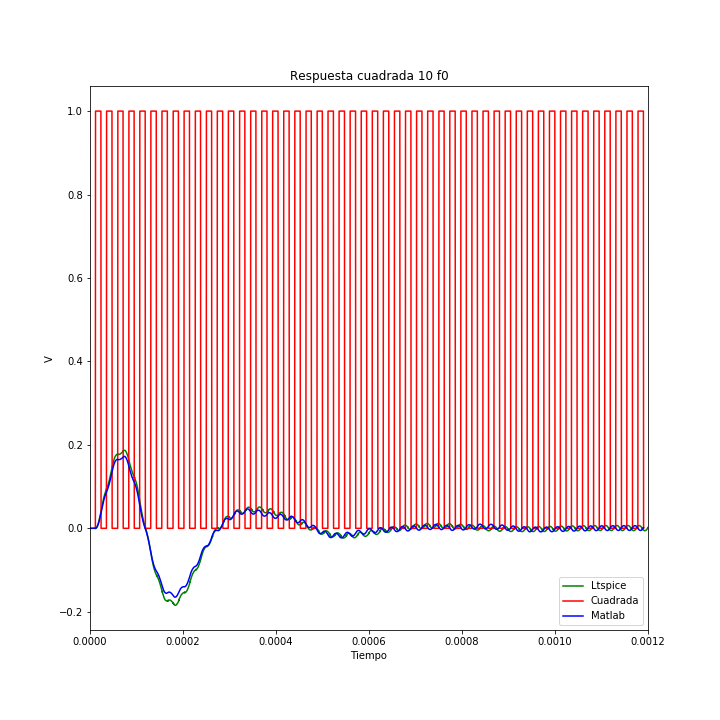
\includegraphics[width=\textwidth]{c_respuesta_cuadrada_por_10.png}
\caption{Simulacion LTspice normalizado vs Matlab}
\break
\end{figure}
\end{itemize}

\end{itemize}


\newpage
\section*{Calculo analitico}
\begin{itemize}
\item Respuesta al impulso\\

\begin{itemize}
	\item p$_{1}$ = -12002.32+34212.9j = -$\alpha_{1}$ + $\beta_{1}$ j\\
	\item $\bar{p_{1}}$ = -12002.32-34212.9j = -$\alpha_{1}$ - $\beta_{1}$ j\\
	\item p$_{2}$ = -5767.68+16439.38j = -$\alpha_{2}$ + $\beta_{2}$ j\\
	\item $\bar{p_{2}}$ = -5767.68-16439.38j = -$\alpha_{2}$ - $\beta_{2}$ j\\
\end{itemize}

\begin{align*}
V_{o}(s) &= H(s) \cdot V_{i}(s)\\[10pt]
V_{i} &= 1 \\[10pt]
V_{o}(s) &= \frac{6,317 \cdot 10^8 \cdot s^2}{(s - p_{1}) \cdot (s - \bar{p_{1}}) \cdot (s - p_{2}) \cdot (s - \bar{p_{2}})} \\[10pt]
V_{o}(s) &= \frac{K_{1}}{(s - p_{1})} + \frac{\bar{K_{1}}}{(s - \bar{p_{1}})} +  \frac{K_{2}}{(s - p_{2})} + \frac{\bar{K_{2}}}{(s - \bar{p_{2}})} \\[10pt]
K_{1} &= 2693 - 12334.70 j \\[10pt]
\bar{K_{1}} &= 2693 + 12334.70 j \\[10pt]
K_{2} &= -2693 + 5436.1 j \\[10pt]
\bar{K_{2}} &= -2693 - 5436.1 j \\[10pt]
\end{align*}

Una vez obtenias las fracciones simples podemos antitransformar y sabemos la siguiente propiedad: \\
\begin{tabular}{ |p{6cm}|p{6cm}|  }
 \hline
 \multicolumn{2}{|c|}{Anti Transformada de Laplace} \\
 \hline
 f(t)& F(s)\\
 \hline
 re$^{- \alpha t}$ $\cdot$ cos($\beta$t + $\theta$) $\cdot$ u(t)  & $\frac{0.5 r ^{j \theta}}{s + a -jb}$ + $\frac{0.5 r ^{-j \theta}}{s + a + jb}$ \\
 \hline
\end{tabular}\\

Entonces la respuesta es:

\begin{align*}
V_{o}(t) = &2 \cdot |K_{1}| \cdot e^{- \alpha_{1} \cdot t} \cdot cos(\beta_{1} \cdot t + Arg(K_{1})) \\
&+  2 \cdot |K_{2}| \cdot e^{- \alpha_{2} \cdot t} \cdot cos(\beta_{2} \cdot t + Arg(K_{2}))\\[10pt]
\end{align*}

\begin{align*}
V_{o}(t) = &2 \cdot 12625.26 \cdot e^{-12002 \cdot t} \cdot cos(34212.9 \cdot t - 1.355) \\
&+  2 \cdot 6066.60 \cdot e^{-5767 \cdot t} \cdot cos(16439.38 \cdot t + 2.030)\\[10pt]
\end{align*}

Aca vemo como el polo con la parte real mas chica (en este caso $\alpha_{2}$ = 5767) es el que estabiliza el sistema.

\newpage
\item Respuesta al escalon
\begin{align*}
V_{o}(s) &= H(s) \cdot V_{i}(s)\\[10pt]
V_{i} &= 1/s \\[10pt]
V_{o}(s) &= \frac{6,317 \cdot 10^8 \cdot s}{(s - p_{1}) \cdot (s - \bar{p_{1}}) \cdot (s - p_{2}) \cdot (s - \bar{p_{2}})} \\[10pt]
V_{o}(s) &= \frac{K_{1}}{(s - p_{1})} + \frac{\bar{K_{1}}}{(s - \bar{p_{1}})} +  \frac{K_{2}}{(s - p_{2})} + \frac{\bar{K_{2}}}{(s - \bar{p_{2}})} \\[10pt]
K_{1} &= -0.3456 + 0.04253j \\[10pt]
\bar{K_{1}} &= -0.3456 - 0.02353j \\[10pt]
K_{2} &= 0.3456 + 0.02353j  \\[10pt]
\bar{K_{2}} &= 0.3456 - 0.02353j  \\[10pt]
\end{align*}

Usando la misma propiedad que para el caso anterior:

Entonces la respuesta es:

\begin{align*}
V_{o}(t) = &2 \cdot |K_{1}| \cdot e^{- \alpha_{1} \cdot t} \cdot cos(\beta_{1} \cdot t + Arg(K_{1})) \\
&+  2 \cdot |K_{2}| \cdot e^{- \alpha_{2} \cdot t} \cdot cos(\beta_{2} \cdot t + Arg(K_{2}))\\
\end{align*}
Reemplazando los valores, nos da lo siguiente:
\begin{align*}
V_{o}(t) = &2 \cdot 0.348 \cdot e^{-12002 \cdot t} \cdot cos(34212.9 \cdot t + 3.019) \\
&+  2 \cdot 0.348 \cdot e^{-5767 \cdot t} \cdot cos(16439.38 \cdot t + 0.122)\\[10pt]
\end{align*}

\newpage
\item Respuesta a la senoidal de una frecuencia:


\begin{align*}
f &= 4200 \\[10pt]
w &= 4200 \cdot 2 \cdot \pi \\[10pt]
p_{w} &= w \cdot (0 + 1j) = 26389.378 j = \beta_{w} j\\[10pt]
\bar{p_{w}} &= w \cdot (0 - 1j)  = -26389.378 j = - \beta_{w} j\\[10pt]
V_{o}(s) &= H(s) \cdot V_{i}(s)\\[10pt]
V_{i} &= \frac{w}{w^{2} + s^{2}} \\[10pt]
V_{o}(s) &= \frac{6,317 \cdot 10^8 \cdot s^2}{(s - p_{1}) \cdot (s - \bar{p_{1}}) \cdot (s - p_{2}) \cdot (s - \bar{p_{2}}) \cdot (s - p_{w}) \cdot (s - \bar{p_{w}})} \\[10pt]
V_{o}(s) &= \frac{K_{1}}{(s - p_{1})} + \frac{\bar{K_{1}}}{(s - \bar{p_{1}})} +  \frac{K_{2}}{(s - p_{2})} + \frac{\bar{K_{2}}}{(s - \bar{p_{2}})} +  \frac{K_{3}}{(s - p_{w})} +  \frac{\bar{K_{3}}}{(s - \bar{p_{w}})}\\[10pt]
K_{1} &= 0.311 + 0.211 j \\[10pt]
\bar{K_{1}} &= 0.311 - 0.211 j \\[10pt]
K_{2} &= -0.242 + 0.212 j \\[10pt]
\bar{K_{2}} &= -0.242 - 0.212 j \\[10pt]
K_{3} &= -0.0689 + 0.495.1 j \\[10pt]
\bar{K_{3}} &= -0.689 - 0.495 j \\[10pt]
\end{align*}

Entonces la respuesta es:

\begin{align*}
V_{o}(t) = &2 \cdot |K_{1}| \cdot e^{- \alpha_{1} \cdot t} \cdot cos(\beta_{1} \cdot t + Arg(K_{1})) \\
&+  2 \cdot |K_{2}| \cdot e^{- \alpha_{2} \cdot t} \cdot cos(\beta_{2} \cdot t + Arg(K_{2}))\\
&+  2 \cdot |K_{3}| \cdot e^{- \alpha_{w} \cdot t} \cdot cos(\beta_{w} \cdot t + Arg(K_{2}))\\
\end{align*}

Pero como $\alpha_{w}$ = 0, entonces: 
\begin{align*}
V_{o}(t) = &2 \cdot |K_{1}| \cdot e^{- \alpha_{1} \cdot t} \cdot cos(\beta_{1} \cdot t + Arg(K_{1})) \\
&+  2 \cdot |K_{2}| \cdot e^{- \alpha_{2} \cdot t} \cdot cos(\beta_{2} \cdot t + Arg(K_{2}))\\
&+  2 \cdot |K_{3}| \cdot cos(\beta_{w} \cdot t + Arg(K_{2}))\\[10pt]
\end{align*}

\end{itemize}

\newpage
Finalmente se dejan los respectivos graficos de cada respuesta calculada analitacamente utilizando 10000 puntos graficando en python.

\begin{figure}[h]
	\centering
	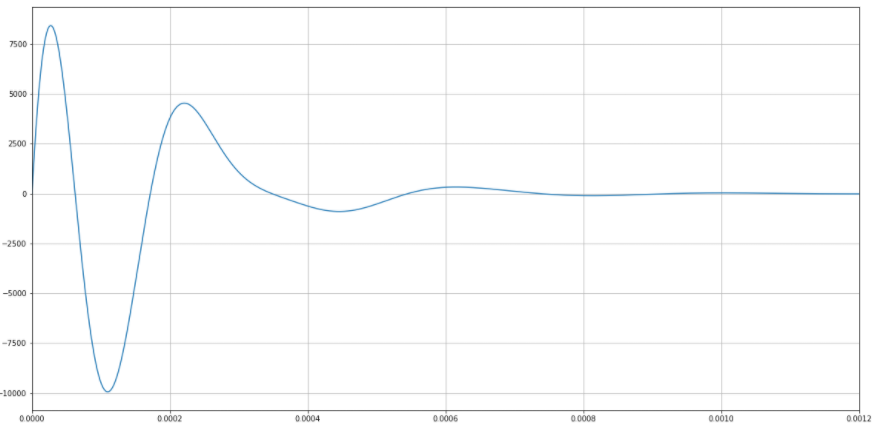
\includegraphics[width=\textwidth]{impulso_python.png}
\caption{Respuesta al impulso analiticamente.}
\end{figure}

\begin{figure}[h]
	\centering
	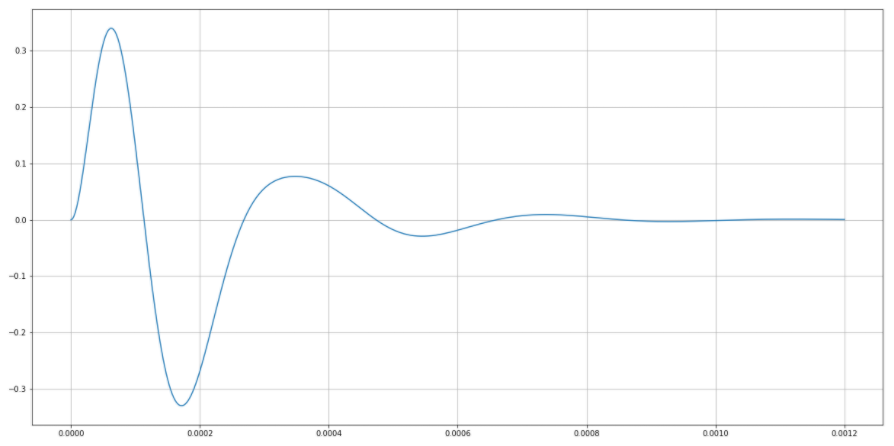
\includegraphics[width=\textwidth]{escalon_python.png}
\caption{Respuesta al escalon analiticamente.}
\end{figure}
\newpage
\begin{figure}[h]
	\centering
	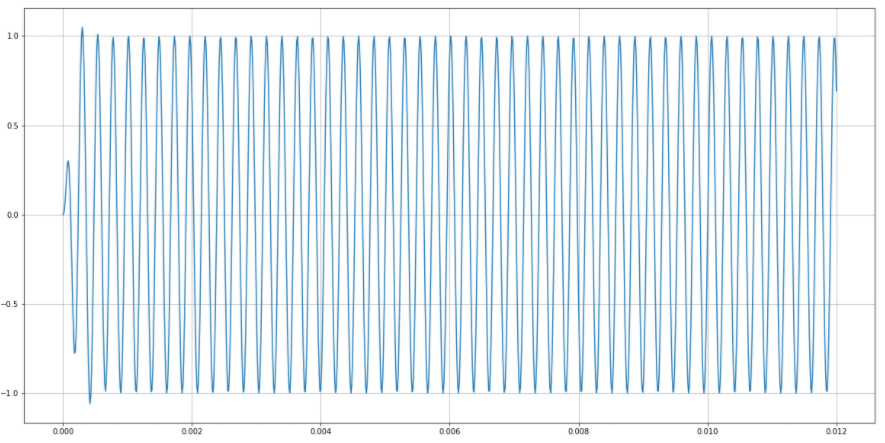
\includegraphics[width=\textwidth]{senoidal_python.png}
\caption{Respuesta a la senoidal (f=4200Hz) analiticamente.}
\end{figure}

%------------------------------------------------

\end{document}
